\documentclass[french,11pt]{article}
\usepackage[utf8]{inputenc}
\usepackage[T1]{fontenc}
\usepackage{babel}
\usepackage{eurosym}
\usepackage[affil-it]{authblk}

\usepackage[table]{xcolor}

\usepackage{tikz}
\usetikzlibrary{arrows,decorations.markings}
\usetikzlibrary{cd}
\usetikzlibrary{shapes.geometric,fit}
\usetikzlibrary{positioning}

\usepackage{leadsheets}

\usepackage[top=4cm, bottom=4cm, left=3cm, right=3cm]{geometry}
\usepackage[fencedCode,inlineFootnotes,citations,definitionLists,hashEnumerators,smartEllipses,hybrid,pipeTables, tableCaptions]{markdown}
\usepackage{keyval}

\usepackage[backend=biber,style=alphabetic,citestyle=authoryear-comp]{biblatex}
\addbibresource{refs.bib}

\usepackage{minted}
\setkeys{Gin}{width=\linewidth,totalheight=\textheight,keepaspectratio}

\usepackage{mathtools}
\usepackage{amsmath}
\usepackage{amsfonts}
\usepackage{amsthm}
\usepackage{amssymb}



\usepackage{graphicx}
\graphicspath{{img/}}
\usepackage{wrapfig}
\usepackage{float}

\usepackage{hyperref}
\interfootnotelinepenalty=10000

\usepackage{setspace}
\onehalfspacing

\usepackage{caption}
\usepackage{subcaption}
\tikzcdset{every label/.append style = {font = \tiny}}

\usepackage{csquotes}
\usepackage{comment}


\usepackage{tabularx}
\definecolor{tableShade}{gray}{0.9}

\usepackage[shortlabels]{enumitem}





\title{LiveScaler}
\author{Alice Rixte}
\begin{document}  

\maketitle

\tableofcontents

\section{Introduction}
\section{Transformations de gammes}
\begin{comment}
  \subsection{Quelles transformations de gamme autoriser ?}
Les transformation affines de la forme $an + b$ où $n$ est la note de départ.
\subsection{Pourquoi ces transformations ?}
\begin{enumerate}
  \item Ces transformations sont adaptées à la musique tonale occidentale : passage du majeur au mineur.
  \item Elles sont facilement implémentables
  \item Elles peuvent être exprimées par une paire d'entiers, ce qui permet de les communiquer directement via MIDI.
\end{enumerate}


\subsection{Peut-on quand même sortir de la tonalité ?}
Oui : \begin{enumerate}
  \item on peut passer d'une gamme quelconque à une gamme par tons
  \item elles s'appliquent dans un contexte microtonal
  \item Possibilité d'ajouter une permutation quelconque personnalisée
\end{enumerate} 
\end{comment}
Dans cet article, on se place dans le contexte des tempéraments à division multiple. On notera $b$ le nombre de divisions de l'octave. Bien que l'ensemble des exemples proposés ici se focalisent sur le tempérament égal $b = 12$, le lecteur se persuadera aisément que tout ce qui est proposé ici peut se généraliser à tous les tempéraments à division multiple. On peut alors associer à toute note un entier $n\in \mathbb{Z}$. En particulier, nous utiliserons ici la norme MIDI en l'étendant à l'ensembles des entiers relatifs : $B_{-2}$ correspond ainsi à $-1$, $C_{-1}$ à $0$, $C\sharp_{-1}$  à $1$, $A_3$ à $57$ \dots

Nous définissons ici une \emph{transformation de gamme} comme une fonction qui à toute hauteur de note associe une nouvelle hauteur de note a priori quelconque, autrement dit une fonction $\mathbb{Z}$ dans $\mathbb{Z}$.

Un bon exemple de transformation de gamme est la transposition : à chaque note $n$ on associe la note $n+\tau$  décalée de $\tau$ demi-tons vers l'aigu lorsque $\tau$ est positif et vers le grave lorsque $\tau$ est négatif. Ainsi, une transposition de $\tau$ demi-tons est représentée par la transformation de gamme $ n \mapsto n+\tau$ (voir Figure \ref{fig:transp}).


\subsection{Transformations affines}

Les transformations de gamme qui vont nous intéresser ici sont les \emph{transformation affines}\footnote{Cette définition est inspirée par les automorphismes du groupe $T/I$ présentés par \textcite{lewin1990klumpenhouwer}.}, c'est-à-dire les fonctions de la forme $A\langle\mu,\tau\rangle : n \mapsto \mu n + \tau$ avec $\mu$ le \emph{coefficient modal} de la transformation affine et $\tau$ le \emph{coefficient de transposition}. 

Les transformations affines ont la propriété importante de préserver les classes de hauteur \footnote{En effet, pour toute base $b\in \mathbb{N}^*$, $\forall n_1,n_2 \in \mathbb{Z}, n_1 \equiv n_2 \mod b \implies \mu n_1 + \tau \equiv \mu n_2 + \tau \mod b$. Avec $b=12$, on obtient le résultat pour les classes de hauteurs dodécaphoniques. }  (au sens de \cite{forte1973structure}) c'est-à-dire que si deux notes sont identiques à l'octave près, alors elles le seront toujours une fois la transformation affine appliquée. 

Nous allons à présent étudier plusieurs exemples afin de donner au lecteur un aperçu de leur expressivité.
\subsubsection{Transpositions}
\begin{figure}[htbp]
  \centering
  \begin{tikzpicture}[baseline= (a).base]    

    \node[scale=1] (a) at (0,0){
    \begin{tikzcd}[column sep=0pt, minimum width=11.5mm, row sep=0.1cm]
    {...} & {A_{-1}} & {A\sharp_{-1}} & {B_{-1}} & {C_{0}} & {C\sharp_{0}} & {D_0} & {D\sharp_0} & {E_0} & {F_0} & {F\sharp_0} & {G_0} & {...} \\
    {...} & {-3} & {-2} & {-1} & 0 & 1 & 2 & 3 & 4 & 5 & 6 & 7 & {...} \\
    {} &&&&&&&&&&& {} \\
    {} &&&&&&&&&&& {} \\
    {} &&&&&&&&&&& {} \\
    {} &&&&&&&&&&& {} \\
    {} &&&&&&&&&&& {} \\
    {} &&&&&&&&&&& {} \\
    {...} & {-3} & {-2} & {-1} & 0 & 1 & 2 & 3 & 4 & 5 & 6 & 7 & {...} \\
    {...} & {A_{-1}} & {A\sharp_{-1}} & {B_{-1}} & {C_0} & {C\sharp_0} & {D_0} & {D\sharp_0} & {E_0} & {F_0} & {F\sharp_0} & {G_0} & {...}
    \arrow[color={rgb,255:red,117;green,117;blue,117}, dotted, from=2-1, to=9-3]
    \arrow[from=2-2, to=9-4]
    \arrow[from=2-3, to=9-5]
    \arrow[from=2-4, to=9-6]
    \arrow[from=2-5, to=9-7]
    \arrow[from=2-6, to=9-8]
    \arrow[from=2-7, to=9-9]
    \arrow[from=2-8, to=9-10]
    \arrow[from=2-9, to=9-11]
    \arrow[from=2-10, to=9-12]
    \arrow[color={rgb,255:red,117;green,117;blue,117}, dotted, from=2-11, to=9-13]
    \end{tikzcd}
  };
  \end{tikzpicture}
  \caption{La transformation $A \langle 1,2 \rangle : n \mapsto n + 2$ correspond à la  transposition d'un ton vers l'aigu}\label{fig:transp}
\end{figure}
Lorsque $\mu = 1$, les transformations affines $A\langle 1,\tau \rangle : n \mapsto n + \tau$ permettent de représenter toutes les transpositions possibles (voir Figure \ref{fig:transp}).


\subsubsection{Inversions}

\begin{figure}[htbp]
  \centering
  \begin{tikzpicture}[baseline= (a).base]

    \node[scale=1] (a) at (0,0){
      \begin{tikzcd}[column sep=0mm, minimum width = 0mm, minimum height=7mm, row sep=0cm]
        \svdots   & \svdots & \hspace{20mm} & \svdots & \svdots \\
        \writechord{G}_{5}  & 7  & & 7  & \writechord{G}_{5}  \\
        \writechord{F#}_{5} & 6  & & 6  & \writechord{F#}_{5} \\
        \writechord{F}_{5}  & 5  & & 5  & \writechord{F}_{5}  \\
        \writechord{E}_{5}  & 4  & & 4  & \writechord{E}_{5}  \\
        \writechord{D#}_{5} & 3  & & 3  & \writechord{D#}_{5} \\
        \writechord{D}_{5}  & 2  & & 2  & \writechord{D}_{5}  \\
        \writechord{C#}_{5} & 1  & & 1  & \writechord{C#}_{5} \\
        \writechord{C}_{5}  & 0  & & 0  & \writechord{C}_{5}  \\
        \writechord{B}_{4}  & -1 & & -1 & \writechord{B}_{4}  \\
        \writechord{A#}_{4} & -2 & & -2 & \writechord{A#}_{4} \\
        \writechord{A}_{4}  & -3 & & -3 & \writechord{A}_{4}  \\
        \svdots         & \svdots & & \svdots &         \svdots 
        \arrow[from=2-2, to=12-4]
        \arrow[from=4-2, to=10-4, color={rgb,255:red,117;green,117;blue,117}, dashed]
        \arrow[from=5-2, to=9-4]
        \arrow[from=7-2, to=7-4, color={rgb,255:red,117;green,117;blue,117}, dashed]
        \arrow[from=9-2, to=5-4]
        \arrow[from=10-2, to=4-4, color={rgb,255:red,117;green,117;blue,117}, dashed]
        \arrow[from=12-2, to=2-4]
      \end{tikzcd}
    };
  \end{tikzpicture}
  \caption{La transformation $A\langle -1,4\rangle :n\mapsto -n + 4$ avec $\alpha =$ \writechord{C}$_5$ et $\beta = 12$}
  \medskip
  \small
  Pour des raisons de lisibilité seules les flèches de la gamme de Do majeur ont été tracées. On notera la passage de l'accord \writechord{Cma} à \writechord{Ami} et de \writechord{Ami} à \writechord{Cma}.
  \label{fig:inversion}
\end{figure}

\begin{figure}
  %\centering
  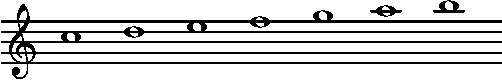
\includegraphics[width=\columnwidth]{c-maj-crop.pdf}
  \begin{tabularx}{\columnwidth}{ YYYYZ }
    &&$ \mathlarger{\mathlarger{\mathlarger{\mathlarger\Downarrow}}}$ & $A\langle -1,4 \rangle$&
    \end{tabularx}
  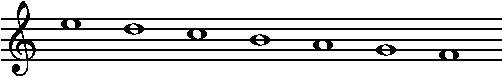
\includegraphics[width=\columnwidth]{e-mod-crop.pdf}
  \caption{L'image de la gamme de Do majeur par $A\langle -1,4 \rangle$ est un mode de Mi}
  \label{fig:modeE}
\end{figure}

Lorsque $\mu = -1$, les transformations $A \langle -1,\tau\rangle : n\mapsto -n + \tau$ permettent de passer d'une gamme majeure à un mode de Mi et réciproquement (voir Figure \ref{fig:modeE}). La Figure \ref{fig:inversion} illustre la manière dont la triade \writechord{C}$_5$, \writechord{E}$_5$, \writechord{G}$_5$ est  par $A\langle -1,4 \rangle$ en la triade \writechord{E}$_5$, \writechord{C}$_5$, \writechord{A}$_4$. De même, l'image de la triade \writechord{A}$_4$, \writechord{C}$_5$, \writechord{E}$_5$  est  \writechord{G}$_5$, \writechord{E}$_5$, \writechord{G}$_5$. Comme les transformations affines préservent les classes de hauteur, on peut affirmer plus généralement que $A \langle -1,4\rangle$ transforme l'accord \writechord{Cma} en \writechord{Ami}   et \writechord{Ami} en \writechord{Cma}. 

Remarquons de plus qu'en changeant l'ancre,  en choisissant $\alpha =$  \writechord{G}$_4$ par exemple, l'image de l'accord \writechord{Gma} par $A\langle-1,4 \rangle$ sera \writechord{Emi}. La Table \ref{tab:triadesA-14} explicite les images des accords de la gamme de Do majeur par $A\langle -1,4 \rangle$ lorsque $\alpha = $ \writechord{C}$_n$ et des accords de la gamme de Sol majeur lorsque l'on change l'ancre pour $\alpha =$ \writechord{G}$_n$, avec $n$ un entier quelconque.


\begin{table}[htbp]
  
  \centering % instead of \begin{center}
  \begin{tabular}{cccccccc}
      \writechord{Cma} & $\mapsto$ & \writechord{Ami} & & & \writechord{Gma} & $\mapsto$ & \writechord{Emi}\\
      \writechord{Dmi} & $\mapsto$ & \writechord{Gma} & & & \writechord{Ami} & $\mapsto$ & \writechord{Dma}\\
      \writechord{Emi} & $\mapsto$ & \writechord{Fma} & & & \writechord{Bmi} & $\mapsto$ & \writechord{Cma}\\
      \writechord{Fma} & $\mapsto$ & \writechord{Emi} & & & \writechord{Cma} & $\mapsto$ & \writechord{Bmi}\\
      \writechord{Gma} & $\mapsto$ & \writechord{Dmi} & & & \writechord{Dma} & $\mapsto$ & \writechord{Ami}\\
      \writechord{Ami} & $\mapsto$ & \writechord{Cma} & & & \writechord{Emi} & $\mapsto$ & \writechord{Gma}\\
      \writechord{Bo} & $\mapsto$ & \writechord{Bo} & & & \writechord{F#o} & $\mapsto$ & \writechord{F#o}
  \end{tabular}
  \caption{Images des accords de la gamme de Do majeur par $A\langle -1, 4 \rangle$ pour $\alpha =$ \writechord{C}$_n$ (à gauche) et de la gamme de Sol majeur pour $\alpha =$ \writechord{G}$_n$ (à droite), pour $n\in\mathbb{Z}$} 
  \label{tab:triadesA-14}
\end{table}

Ainsi, en se basant sur l'image de l'accord majeur dont la tonique correspond à l'ancre, nous pouvons associer les transformations affines pour lesquelle $\mu = 1$ ou $\mu=-1$ au degré de l'image de cet accord dans la gamme. Par exemple, $A\langle -1,4 \rangle$ peut être associée au degré \writechord{vi} car elle associe le sixième degré mineur à  l'accord majeur dont la tonique est l'ancre (\writechord{Ami} pour \writechord{Cma}, \writechord{Emi} pour \writechord{Gma}, \dots). On obtient ainsi une notation plus intuitive que la notation mathématique, dont la table \ref{tab:degrees} donne un aperçu. 

\begin{table}[htbp]
  \centering
  \rowcolors{2}{gray!25}{white}
  \begin{tabular}{ccc}
    \rowcolor{gray!50}
    Degré & Transformation affine\\
    \writechord{I} & $A\langle ~~1, ~~0\rangle$\\
    \writechord{ii} &  $A\langle -1, -3 \rangle$\\
    \writechord{iii} &  $A\langle -1, -1 \rangle$\\
    \writechord{IV} &  $A\langle ~~1,~~ 5 \rangle$\\
    \writechord{V} &  $A\langle ~~ 1, ~~7 \rangle$\\
    \writechord{vi}& $A\langle -1, ~~4\rangle$\\
    \writechord{vii} & $A\langle -1, ~~6 \rangle$\\
  \end{tabular}
  \caption{ Correspondances entre triades d'une gamme majeure et transformations de gamme\label{tab:degrees} } 
\end{table}

Remarquons que, de manière générale, les inversions affines se comportent moins bien sur les modes non naturels. Par exemple, $A\langle -1, 4\rangle ($\writechord{G\sharp}$) = $ \writechord{G\sharp} donc l'image de la gamme de La mineur harmonique par $A\langle -1, 4\rangle$ contient les notes \writechord{C}, \writechord{D}, \writechord{E}, \writechord{F}, \writechord{G}, \writechord{G\sharp}, \writechord{B}, ce qui ne correspond pas à un mode standard de la musique tonale. C'est une des faiblesses des transformations affines.

\subsubsection{Transformation vers une gamme par ton}
Lorsque $\mu = 2$ ou $\mu = -2$, les transformations affines envoient n'importe quelle gamme vers une gamme apparentée à une gamme par tons (voir Figure \ref{fig:gammepartons}). Les transformations affines peuvent donc permettre de sortir du cadre de la musique tonale occidentale.

\begin{figure}[htbp]
  \centering
  \begin{tikzpicture}[baseline= (a).base]    

    \node[scale=1] (a) at (0,0){
    \begin{tikzcd}[column sep=0pt, minimum width=11.5mm, row sep=0.1cm]
    \dots & G_{-2} & G\sharp_{-2} & A_{-2} & A\sharp_{-2} & B_{-2} & C_{-1} & C\sharp_{-1} & D_{-1} & D\sharp_{-1} & E_{-1} & F_{-1}  & \dots \\
      \dots & -5 &-4 & -3 & -2 & -1 & 0 & 1 & 2 & 3 & 4 & 5 &  \dots \\
      {} &&&&&&&&&&& {} \\
      {} &&&&&&&&&&& {} \\
      {} &&&&&&&&&&& {} \\
      {} &&&&&&&&&&& {} \\
      {} &&&&&&&&&&& {} \\
      {} &&&&&&&&&&& {} \\
      \dots & -5 &-4 & -3 & -2 & -1 & 0 & 1 & 2 & 3 & 4 & 5 &  \dots \\
      \dots & G_{-2} & G\sharp_{-2} & A_{-2} & A\sharp_{-2} & B_{-2} & C_{-1} & C\sharp_{-1} & D_{-1} & D\sharp_{-1} & E_{-1} & F_{-1} & \dots \\
      \arrow[color={rgb,255:red,117;green,117;blue,117}, dotted, from=2-4, to=9-1]
      \arrow[from=2-5, to=9-3]
      \arrow[from=2-6, to=9-5]
      \arrow[from=2-7, to=9-7]
      \arrow[from=2-8, to=9-9]
      \arrow[from=2-9, to=9-11]
      \arrow[color={rgb,255:red,117;green,117;blue,117}, dotted,from=2-10, to=9-13]
      %\arrow[color={rgb,255:red,117;green,117;blue,117}, dotted, from=2-11, to=9-15]
      %\arrow[from=2-9, to=9-3]
      %\arrow[from=2-10, to=9-3]
    \end{tikzcd}
    };
  \end{tikzpicture}   
  \caption{La transformation $A\langle 2,0\rangle :n\mapsto 2n$ permet d'obtenir des gammes apparentées à la gamme par tons.\label{fig:gammepartons}}
\end{figure}

Contrairement aux inversions et aux transpositions, cette transformation n'est pas bijective : l'image de $A\langle 2,0 \rangle$ contient exactement $6$ classes de hauteurs qui correspondent aux $6$ notes d'une des deux gammes par tons. Il est intéressant de noter que l'image d'une gamme majeure ou mineure naturelle par $A\langle 2,\tau\rangle$ contient les $6$ notes de la gamme par tons (voir Table \ref{tab:minparton}). Ce n'est pas le cas pour la gamme mineure harmonique dont l'image par $A\langle 2,\tau\rangle$ ne contient que $5$ classes de hauteur.




\begin{table}[htbp]
  \centering
  \begin{subtable}{0.45\textwidth}
    \centering % instead of \begin{center}
      \begin{tabular}{ccc}
          \writechord{C} & $\mapsto$ & \writechord{C}\\
          \writechord{D} & $\mapsto$ & \writechord{E}\\
          \writechord{E} & $\mapsto$ & \writechord{G\sharp}\\
          \writechord{F} & $\mapsto$ & \writechord{A\sharp}\\
          \writechord{G} & $\mapsto$ & \writechord{D}\\
          \writechord{A} & $\mapsto$ & \writechord{F\sharp}\\
          \writechord{B} & $\mapsto$ & \writechord{A\sharp}
      \end{tabular}
  \end{subtable}
  \begin{subtable}{0.45\textwidth}
      \centering % instead of \begin{center}
      \begin{tabular}{ccc}
          \writechord{C} & $\mapsto$ & \writechord{C}\\
          \writechord{D} & $\mapsto$ & \writechord{E}\\
          \writechord{E\flat} & $\mapsto$ & \writechord{F\sharp}\\
          \writechord{F} & $\mapsto$ & \writechord{A\sharp}\\
          \writechord{G} & $\mapsto$ & \writechord{D}\\
          \writechord{A\flat} & $\mapsto$ & \writechord{E}\\
          \writechord{B\flat} & $\mapsto$ & \writechord{G\sharp}
      \end{tabular}
    \end{subtable}
    \caption{Image des gammes de Do majeur (à gauche) et Do mineur (à droite) par $A\langle 2, 0 \rangle$\label{tab:minparton}}
\end{table}
\subsubsection{Coefficient modal}

La Table \ref{tab:classmu} résume les différents types de transformations qu'offrent les transformations affines, ainsi que le nombre de classes de hauteur dans l'image de ces transformations \footnote{On montre aisément que le nombre de classes de hauteur dans l'image de $A\langle \mu, \tau\rangle$ est égal à $\frac{12}{\mu\wedge 12}$ où $\wedge$ dénote le pgcd de deux entiers.}. Les transformations affines bijectives - leur image contient $12$ classes de hauteurs - correspondent  aux automorphismes $F\langle u,j \rangle$ du groupe $T/I$ décrits par \cite{lewin1990klumpenhouwer}.


\begin{table}[h]
  \centering
  \rowcolors{2}{gray!25}{white}
  \begin{tabular}{ccc}
    \rowcolor{gray!50}
    $\mu$ & Type de transformation & Classes de hauteur\\
    -1 & Inversions majeur/mineur & 12\\
    0 & Octaves & 1\\
    1 & Transpositions & 12 \\
    -2,2 & Gamme par tons & 6 \\
    -3,3 & Tierces mineures &4 \\
    -4,4 & Tierces majeures & 3\\
    -5,5 & $F\langle 5,\tau \rangle$, $F\langle 7,\tau \rangle$& 12 \\
    -6,6 & Tritons & 2\\
  \end{tabular}
  \caption{Classification des transformations affines en fonction de leur coefficient modal $\mu$\label{tab:classmu} } 
\end{table}
\subsection{Restriction de l'écart de hauteur}
Jusqu'ici, nous avons présenté les transformations affines en nous concentrant sur leur action sur les classes de hauteur. Dans la pratique, si nous appliquons directement $A\langle -1,4 \rangle$ à la note  $\writechord{A}_3$ qui correspond au La 440Hz et à la note MIDI $53$, on obtient $A\langle -1,4 \rangle(\writechord{A}_3) = A\langle -1,4 \rangle(57) = -53 = \writechord{G}_{-5}$, qui est bien trop grave pour être audible. 

Afin d'éviter de sortir de la tessiture de l'instrument, ou même du spectre auditif, nous allons restreindre l'écart entre la note initiale et son image par une transformation de gamme quelconque $T : \mathbb{Z}\rightarrow \mathbb{Z}$. On souhaite alors définir à partir de $T$ une nouvelle transformation $T\langle \beta^-, \beta^+\rangle : \mathbb{Z}\rightarrow \mathbb{Z}$ telle que $ - \beta^- \leq T\langle \beta^-, \beta^+\rangle(n) \leq \beta ^+$, où $\beta^+$ (resp. $\beta^-$) est l'interval montant (resp. descendant) maximum entre la note initiale et son image.

Posons $\beta = \beta^- + \beta^+$.  Dans la plupart des cas on souhaite que $\beta = b = 12$ , mais il peut être intéressant de choisir par exemple $\beta  = 2b$, pour préserver le caractère montant ou descendant d'une ligne mélodique.

Soit $r = |T(n) - n | \mod b$ le reste de la division euclidienne de  $|T(n) - n |$ par $b$. On pose alors 
$$
T\langle b, \beta^+, \beta^- \rangle : n \mapsto \begin{cases}
  n + r & \text{si $r \leq \beta^+$}\\
  n + r - \beta & \text{sinon}
\end{cases}
$$

Nous pouvons maintenant appliquer cette restriction de l'intervalle de hauteur à nos fonctions affines. On obtient alors un sous-ensemble contraint de transformations de gamme de la forme $A\langle \mu, \tau, \alpha, b, \beta^-, \beta^+\rangle$. Ce sont exactement ces transformations qui sont implémentées dans Live Scaler.
  


\subsection{Ancres}

Les paramètres des transformations $A\langle \mu, \tau \rangle$ dépendent de la tonalité dans laquelle on se trouve. Ainsi le passage à le relative mineure est $A\langle -1,4 \rangle$ lorsque la tonalité est Do majeur mais correspond à $A\langle -1,6 \rangle$ lorsqu'on est en Sol majeur.

Pour éviter les confusions, on ajoute un troisième paramètre $\alpha$, appelé \emph{ancre} à nos transformations affines. L'ancre correspond à la note qui sert de référence pour appliquer la transformation affine considérée, c'est-à-dire à $0$ dans l'espace $\mathbb{Z}$ des hauteurs de notes. Pour une transformation quelconqe $T:\mathbb{Z} \rightarrow \mathbb{Z}$ et une ancre $\alpha$, on obtient une nouvelle transformation $T\langle \alpha \rangle = A\langle 1, \alpha \rangle \circ T \circ A\langle 1, -\alpha \rangle $ centrée en $\alpha$. 



S'il est clair que les ancres n'ajoutent aucune expressivité à nos transformations affines, elles permettent de rendre la modulation et la transposition avec LiveScaler extrêmement intuitives. En prenant pour référence une gamme majeure dont la tonique est donnée par l'ancre $\alpha$, nous pouvons nommer certaines transformations affines en fonction de l'image de l'accord de tonique. Ainsi les transpositions de $7$ demi-tons vers le haut  $A\langle 1, 7, \alpha\rangle$ envoient l'accord de tonique sur l'accord de dominante et sont donc notées \emph{V}. Le passage à la relative mineure $A\langle -1, 4, \alpha \rangle$ correspond ainsi à \emph{vi}. La Table \ref{tab:degrees} donne les transformations affines pour chaque triade d'une gamme majeure.

\begin{table}[htbp]
  \centering
  \rowcolors{2}{gray!25}{white}
  \begin{tabular}{ccc}
    \rowcolor{gray!50}
    Degré & Transformation affine\\
    \writechord{I} & $A\langle ~~1, ~~0, \alpha \rangle$\\
    \writechord{II} &  $A\langle ~~1, ~~2, \alpha \rangle$\\
    \writechord{iii} &  $A\langle -1, -1, \alpha \rangle$\\
    \writechord{IV} &  $A\langle ~~1,~~ 5, \alpha \rangle$\\
    \writechord{V} &  $A\langle ~~ 1, ~~7, \alpha \rangle$\\
    \writechord{vi}& $A\langle -1, ~~4, \alpha \rangle$\\
    \writechord{vii} & $A\langle -1, ~~6, \alpha \rangle$\\
  \end{tabular}
  \caption{ Correspondances entre triades d'une gamme majeure et transformations de gamme\label{tab:degrees} } 
\end{table}







  

\section{Implémentation des transformations de gamme : LiveScaler}

\subsection{Comment appliquer la transformation ?}
Architecture chef d'orchestre/ instrument : 
\begin{enumerate}
  \item Un seul changement de gamme est envoyé à tous les instruments simultanément
  \item Chaque instrument applique la transformation selon ses propres paramètres (e.g. intervalle de repliement)
  \item Deux types de paramètres : \begin{itemize}
    \item Paramètres globaux envoyés sous la forme de messages à tous les instruments sous forme de message. Par exemple : coefficients de la transformation affine.
    \item Paramètre local propre à chaque instrument d'interprétation des messages reçus. Par exemple : intervalle de repliement pour rester dans la tessiture de l'instrument.
    \end{itemize}
\end{enumerate}

\subsection{Quand appliquer la transformation ? }
Instantanément, car le flux MIDI en entrée fait office de "quantize".  ===> Quid des notes en cours ?
\begin{enumerate}
  \item On les arrête
  \item Legato
  \item Retrigger
\end{enumerate}
===> Le choix se fait séparément pour chaque instrument (paramètre local)


\subsection{Justification du choix M4L /Ableton Live}
L'architecture décrite précédemment est présentée comme un paradigme général, on présente ici l'implémentation concrète.
\begin{enumerate}
  \item Outil populaire dans le domaine de l'EDM
  \item Facilité d'utilisation et intégration dans un environnement 
  \item Prototypage aisé dans M4L
  \item Communication entre les entités d'Ableton Live via messages M4L
\end{enumerate}
On pourrait aisément rendre l'usage plus général en codant un couple de VST fonctionnant sur le même principe.

\section{Performance live }
\subsection{Mapping sur le contrôleur MIDI ATOM}
L'objectif est de pouvoir communiquer une transformation affine via un contrôleur MIDI en un seul geste musical.

\begin{figure}[htbp]
  \centering
  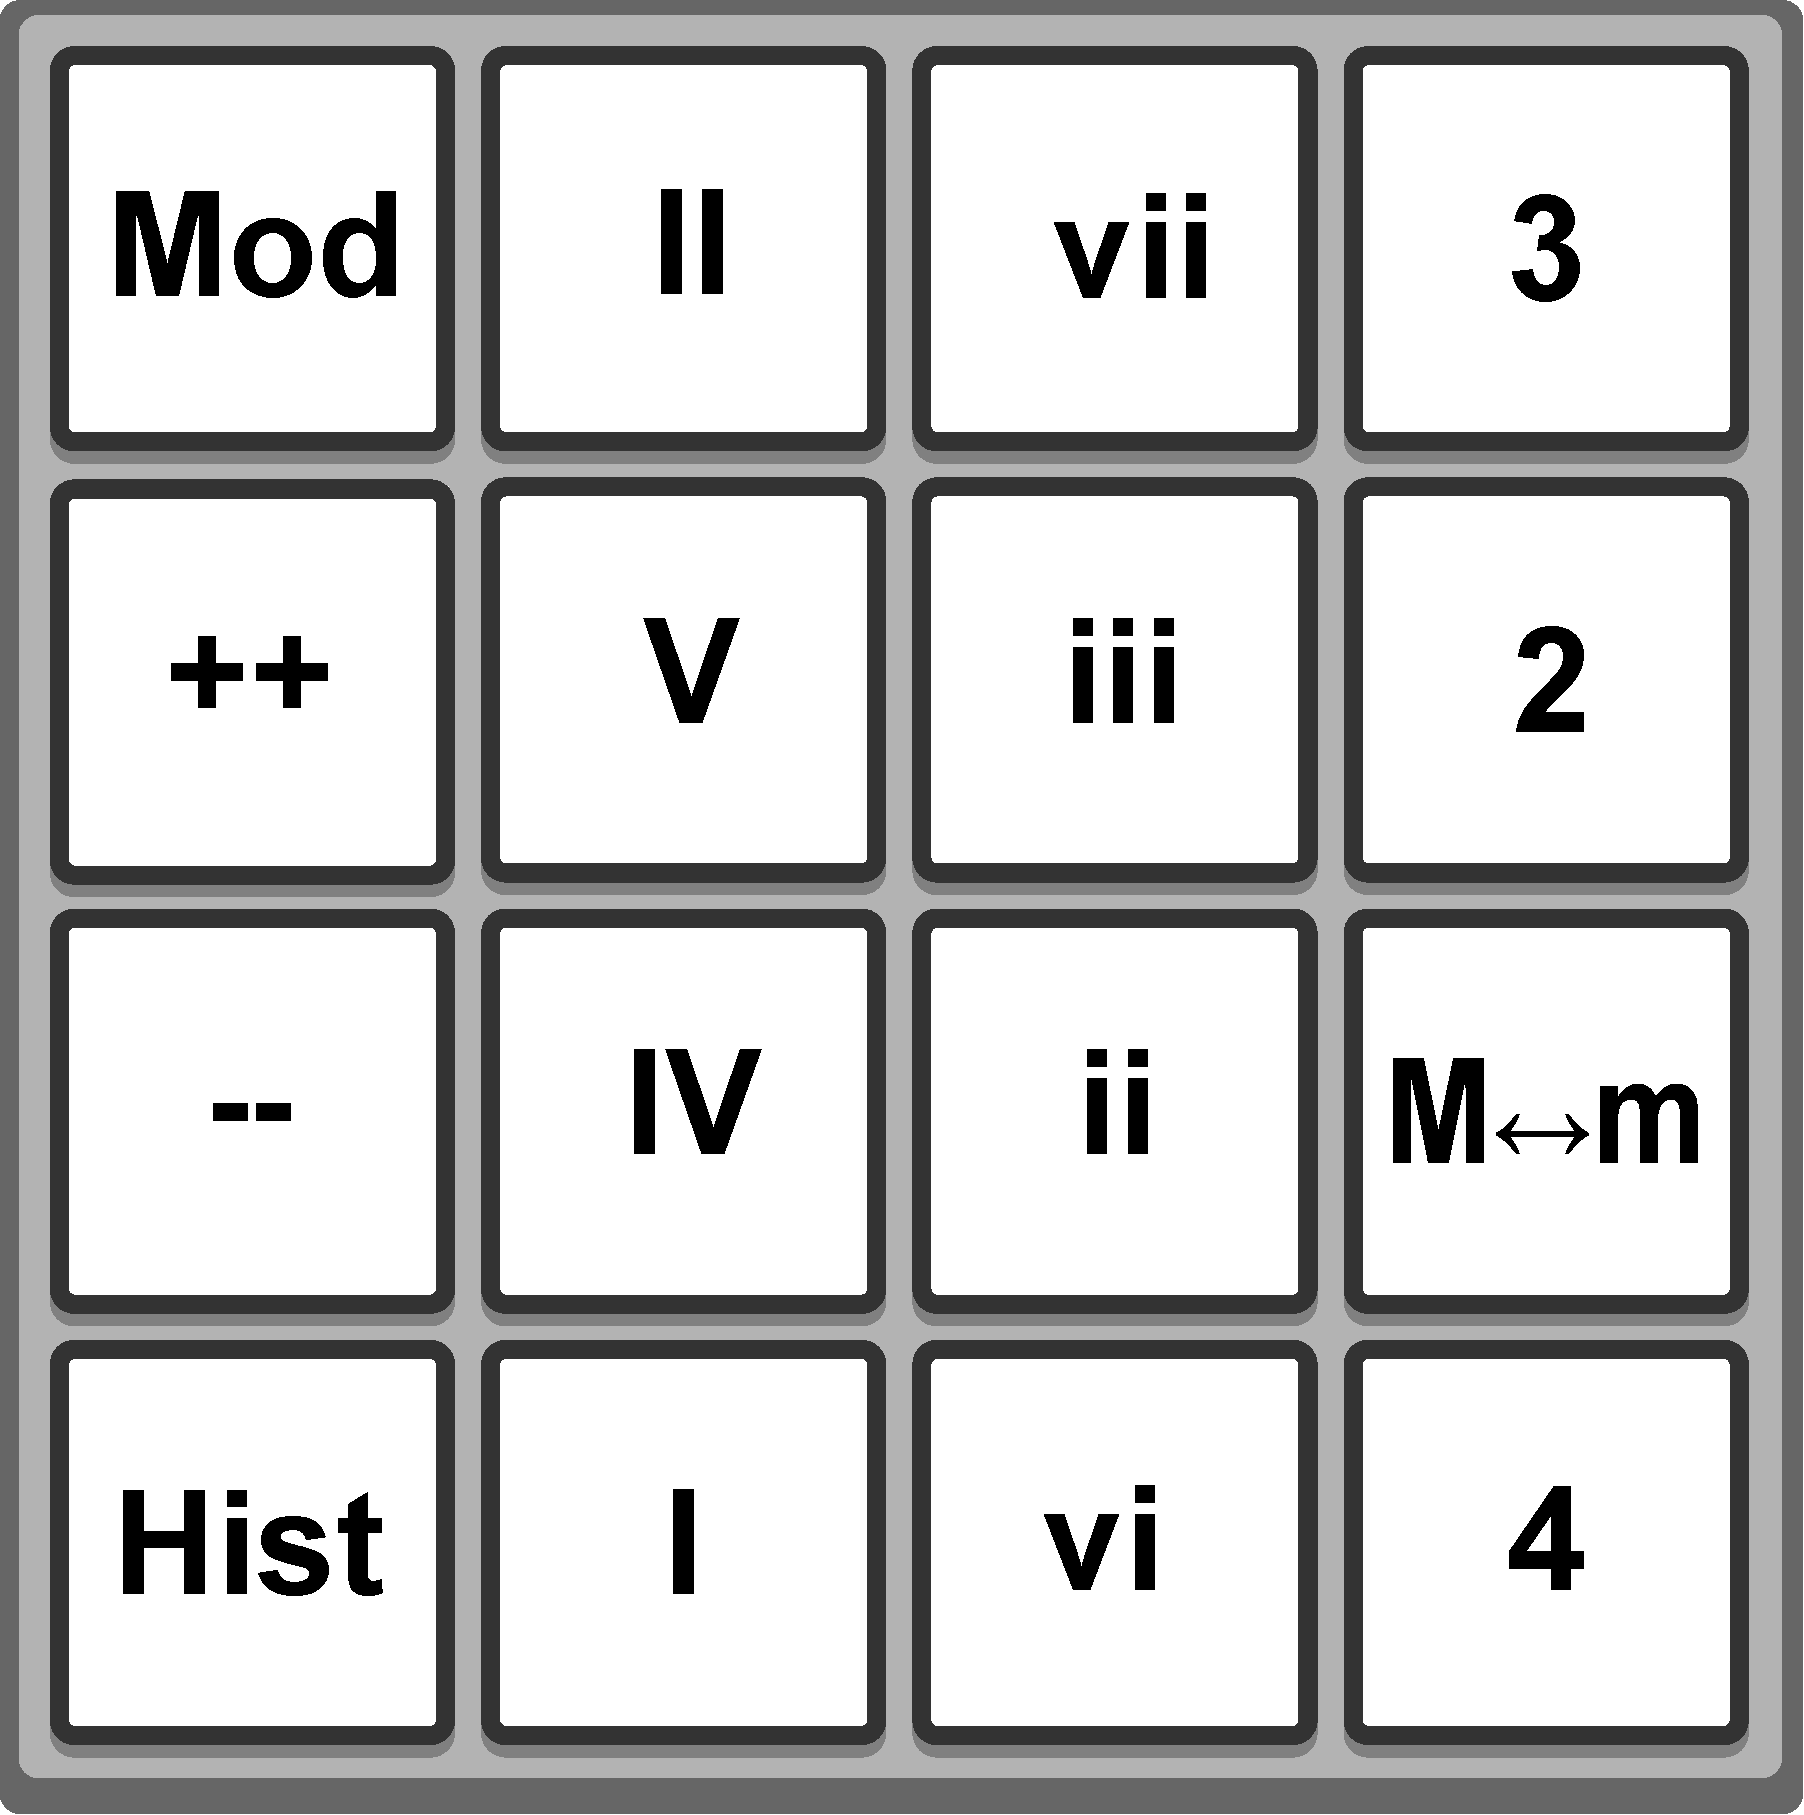
\includegraphics[width=0.55\textwidth]{Figures/Pads-config.pdf}
  \caption{Mapping de Live Scaler sur un contrôleur MIDI à $4\times 4$ pads}
\end{figure}
\begin{enumerate}
  \item Les distances sur le tonnetz sont similaires aux distances entre les pads
  \item Possibilité d'utilisation mélodique (on peut aisément jouer une gamme)
  \item Ancre : transposition et modulations (ajouter au cadre théorique ?)
  \item Historique : revenir aisément en arrière
\end{enumerate}

\subsection{Contrôle de la structure du morceau grâce à Push 2 et Ableton Live}
Séparation de la structure (Push 2) et de l'harmonie ATOM

\begin{figure}[htbp]
  \centering
  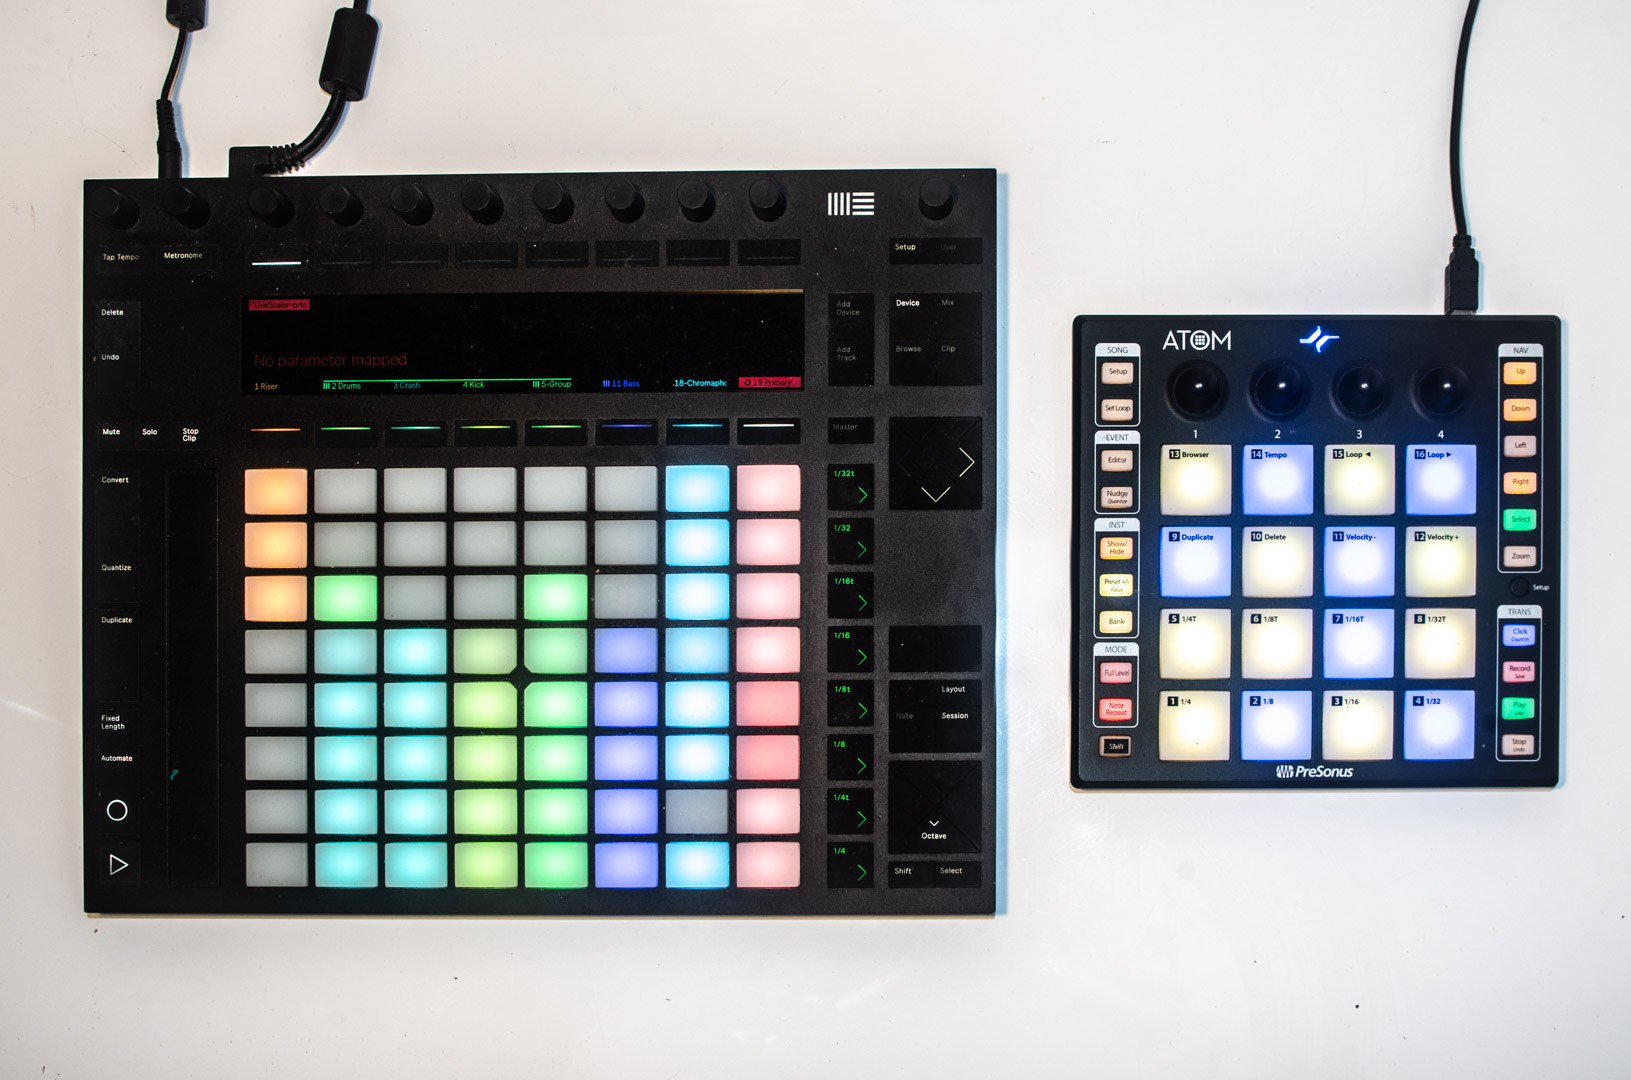
\includegraphics[width=\textwidth]{Figures/IMGP9899.jpg}
  \caption{Contrôleurs MIDI utilisés pour la performance live : à gauche le Push 2 par Ableton (contrôle de la structure du morceau) et à droite ATOM par Presonus (contrôle de l'harmonie du morceau).}
\end{figure}

\subsection{Contraintes sur la composition}
Liste des contraintes :
\begin{enumerate}
  \item Toutes les pistes doivent être MIDI : une piste audio ne serait pas impactée par les changements de gamme
  \item Pauvreté harmonique : le morceau doit être relativement pauvre harmoniquement, idéalement rester sur le même accord tout le long.
\end{enumerate}
Préparation d'une session pour utiliser Live Scaler
\begin{enumerate}
  \item Passer toutes les pistes en MIDI (utiliser des sampleurs pour les pistes audio )
  \item S'assurer qu'on ne sort pas de la tessiture des instruments
  \item Mettre les synthétiseurs et sampleurs en mode legato au maximum.
\end{enumerate}
\subsection{Retour d'expérience}
\begin{enumerate}
  \item Anticiper ses gestes : la transformation de gamme doit être prise en compte avant le moment précis où l'on souhaite qu'elle arrive. Peut devenir très technique assez rapidement
  \item Il est possible de faire concorder le geste avec le changement de gamme (malgré la latence et la faible avance nécessaire) : avantage par rapport au public
  \item Live Scaler est particulièrement adapté à la psytrance et à l'EDM, qui sont initialement harmoniquement pauvre.
\end{enumerate}


\section{Travaux connexes}
\subsection{Transformations de gamme en live coding}
\begin{enumerate}
  \item propositions de Tidal
  \item algorave
\end{enumerate}
\subsection{Théorie transformationnelle}
\begin{enumerate}
  \item Les transformations affines sont une généralisation 
  \begin{enumerate}
    \item des Tonnetz
    \item des k-Nets
  \end{enumerate}
  \item ces transformations sont étudiées et utilisées surtout dans un contexte d'analyse et d'aide à la composition (OpenMusic)
\end{enumerate}

\subsection{Macro contrôle d'un morceau de musique électronique}
\begin{enumerate}
  \item "Changing musical emotion"
\end{enumerate}

\section{Conclusion}
\subsection{Perpectives}
\begin{enumerate}
  \item Associer les changements de gammes à un contrôle d'image (VJing)
  \item Proposer un macro contrôle pour le rythme
  \item Obtenir le retour utilisateurs de musiciens et performeurs
\end{enumerate}
\newpage
\printbibliography


\end{document}
